\chapter{UVic work}
\label{chap:uvicwrk}

\section{Magnetic field testing}

	In Phase~II of BEAST~II, most of the components of Belle~II will be in place, and the magnetic field will be turned on. It was thus necessary to determine whether or not the He-3 tubes would be affected by the magnetic field, or if they would distort the field in an undesirable way. To test this, a single horseshoe magnet was placed with its poles pointing upward. A gaussmeter probe, supported by a lab stand, was placed between the poles. A He-3 tube, also supported by a lab stand, was placed in various locations near the probe, as seen in Fig~\ref{fig:apparatusSchematic}.

\begin{figure}[htb]
	\centering
	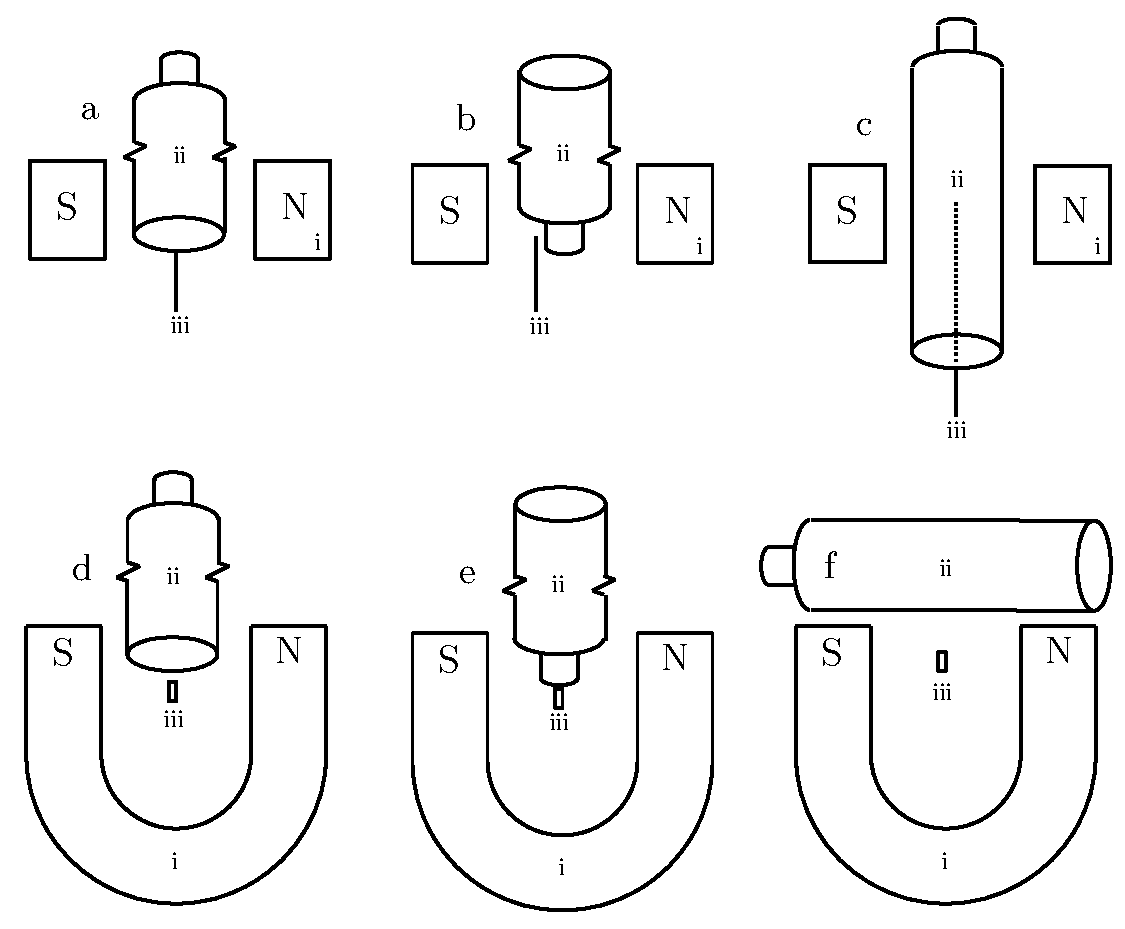
\includegraphics[width=5in]{images/Apparatus_III}
	\caption{Schematic of neutron detector and gaussmeter probe placement (not to scale)}	
	\label{fig:apparatusSchematic}
\end{figure}

Results of the experiment can be found in Table~\ref{tab:magField}. From the results of this test, we can conclude that the detector is non-magnetic.

\begin{table}[ht]
	\centering
	\begin{tabular}{ lll }
		Position & Field without He-3 tube present (kG) & Field with He-3 tube present (kG) 	\\ \hline \hline
		a & 1.322 & 1.321 \\			
		b & 1.321 & 1.319 \\			
		c & 1.322 & 1.322 \\			
		d & 1.323 & 1.321 \\				
		e & 1.323 & 1.314 \\		
		f & 1.489 & 1.489 \\		\hline	
	\end{tabular}
	\caption{Results of magnetic field test}
	\label{tab:magField}
\end{table}


\clearpage
\section{source room}

	The detectors will be plateaued using this source in order to find the working voltage. One of the devices has already been plateaued.

\begin{figure}[htb]
	\centerfloat
	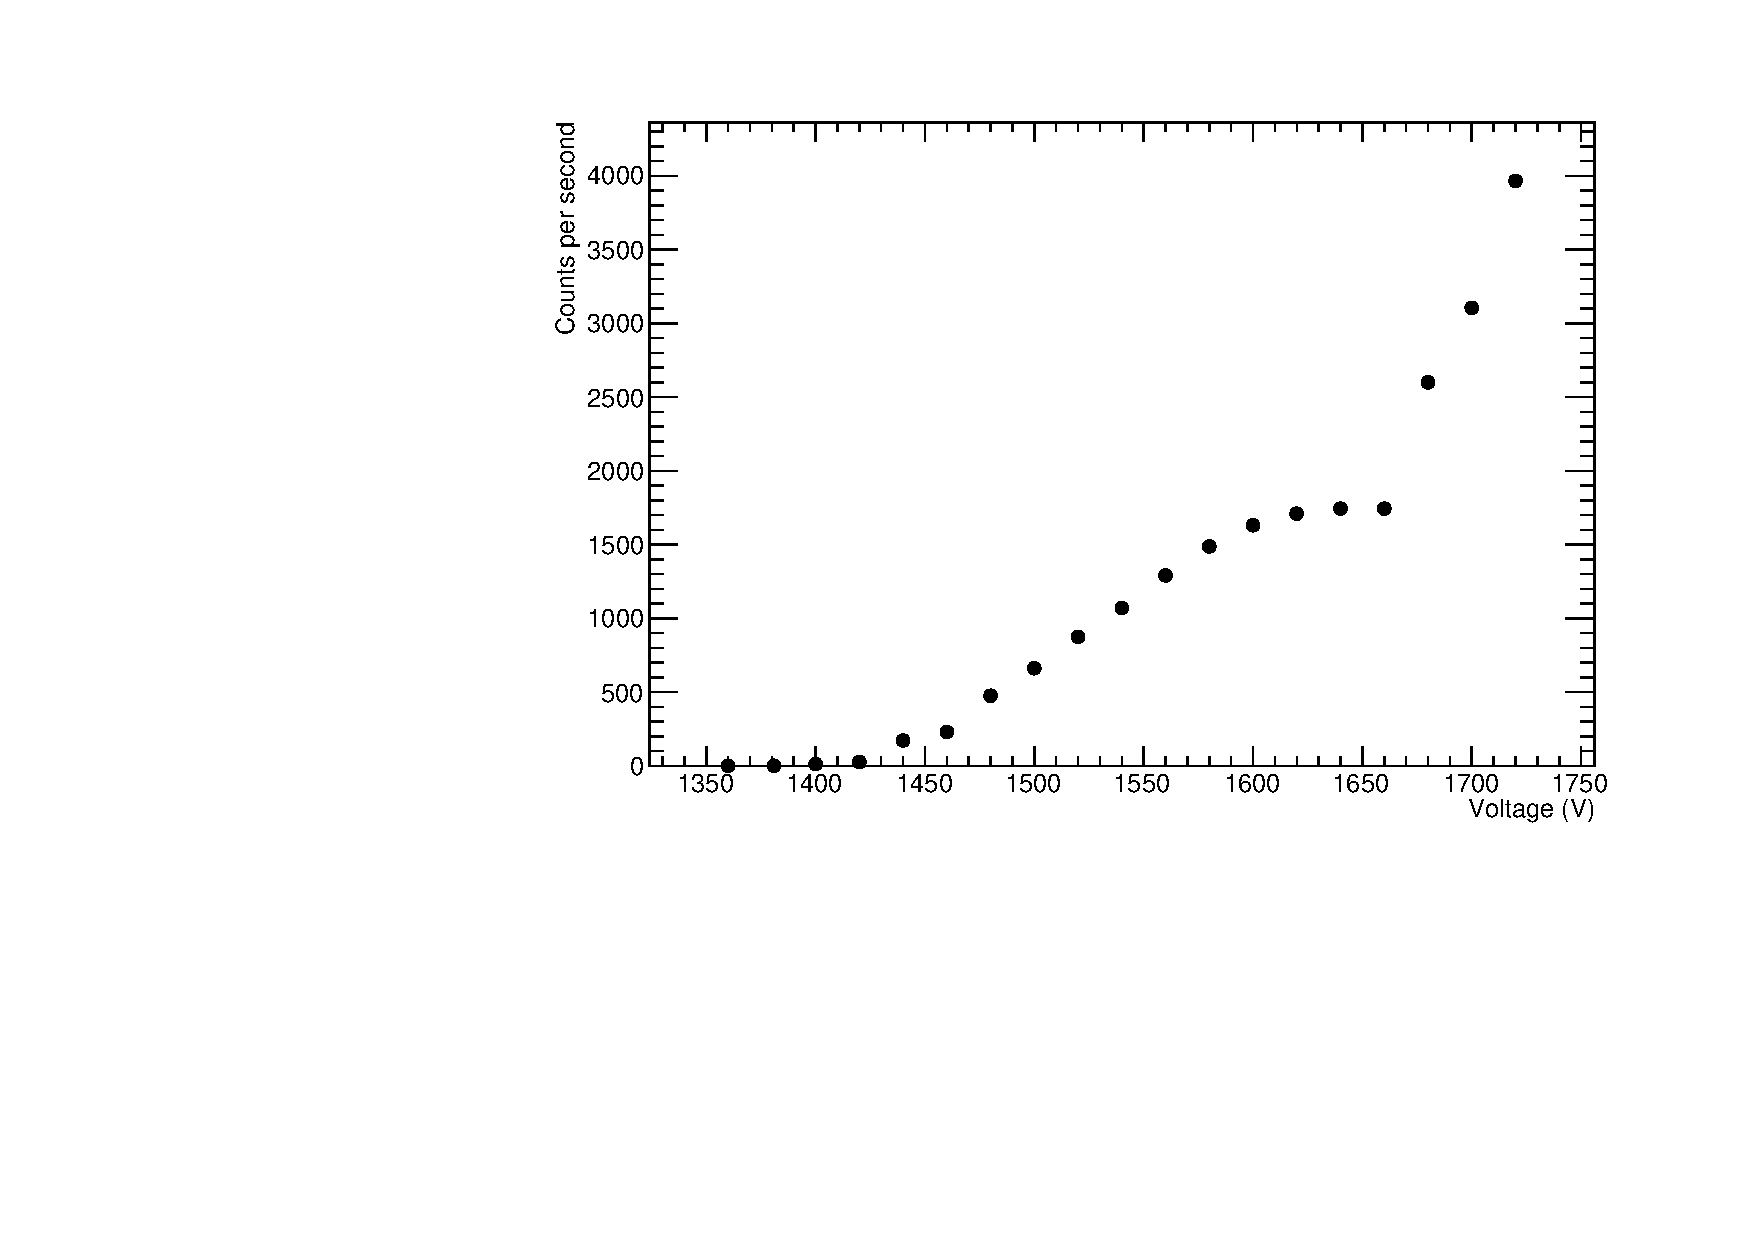
\includegraphics[width=6in]{images/Plateau}
	\caption{Plateau curve for He-3 tube}	
	\label{fig:PlateauCurve}
\end{figure}


Another part of the testing was seeing what the effect of placing various materials between the detector and the neutron source. The materials used were borax, paraffin wax, and polyethylene. For these tests, the detector remained in one place, and the shielding materials were stacked around them. Photographs of the arrangement can be found in Fig~\ref{fig:matTest}. Table~\ref{tab:matTest} summarized the change in rate measured by the detector for each material. Note that the coverage by each material is not equal.

\begin{table}[ht]
	\centering
	\begin{tabular}{ llll }
		Material 	& Density ($g/cm^3$)	& Thickness ($cm$) & Count rate ($Hz$)\\ \hline\hline
		Nothing  	& - 			& - 		 & 6895.2	\\
		Borax	 	& 1.73 			& 5.0		 & 2254.5   	\\
		Paraffin Wax 	& 0.90 			& 11.8		 & 1768.9   	\\
		Polyethylene 	& 0.94 			& 7.5		 & 592.1	\\
		All	 	& 1.39*			& 24.3 		 & 194.0	\\ \hline
		* Mean, Weighted by thickness
	\end{tabular}
	\caption{Count rate for various shielding materials}
	\label{tab:matTest}
\end{table}	



\clearpage
\begin{figure}[hbt]
	\centerfloat
	\subfigure[Nothing]{
		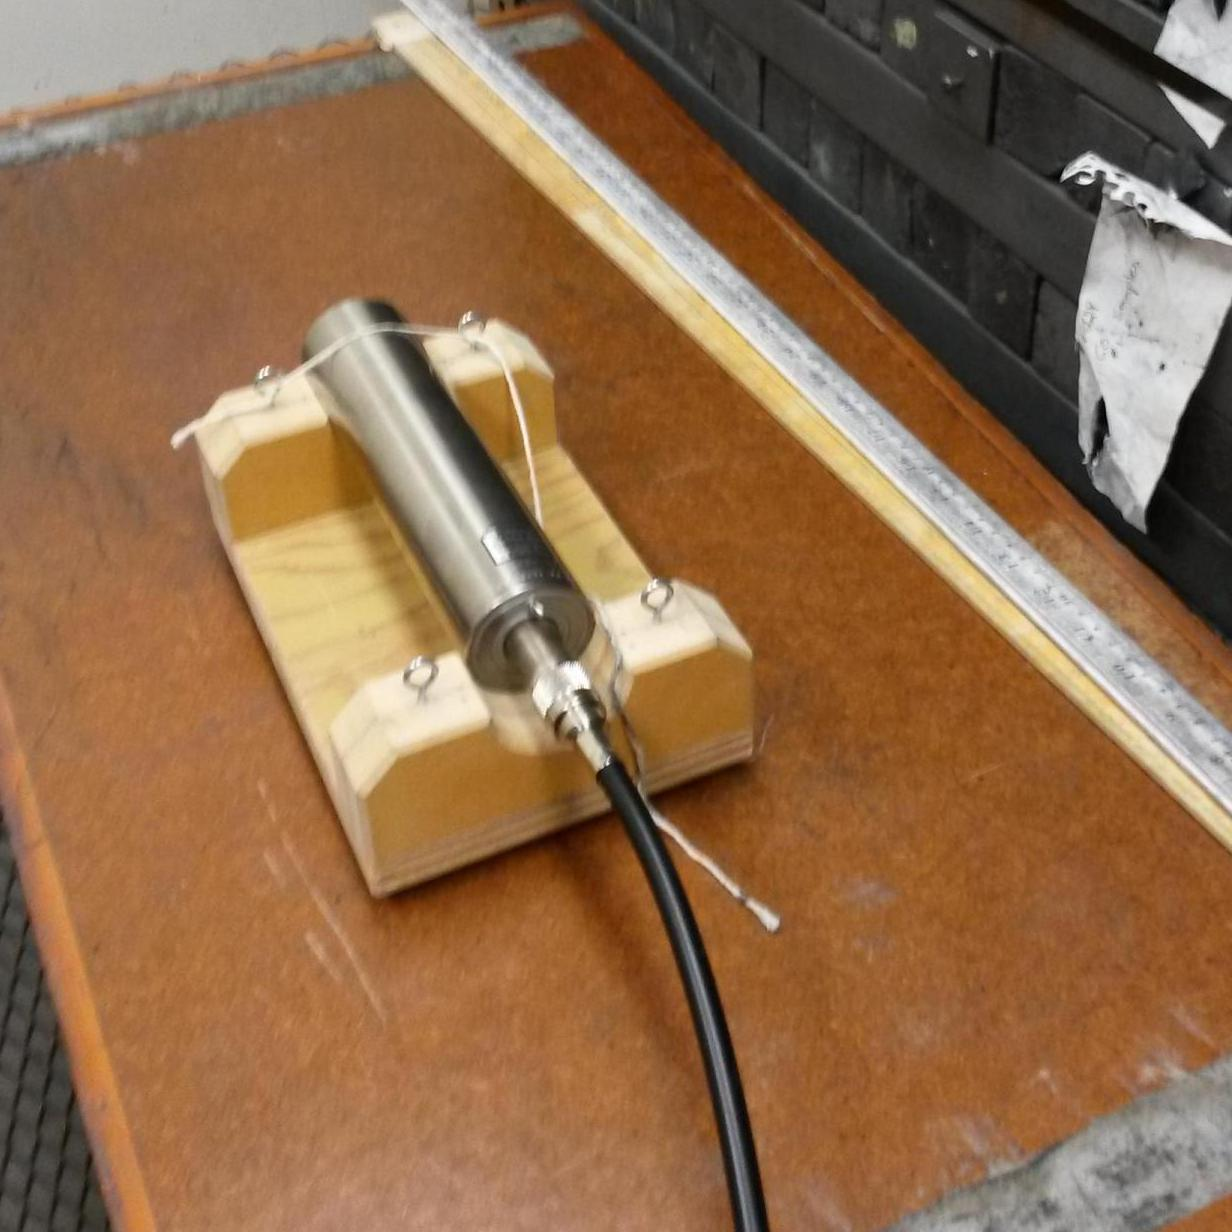
\includegraphics[scale=0.2]{images/Nothing}
	}
	\subfigure[Borax]{
		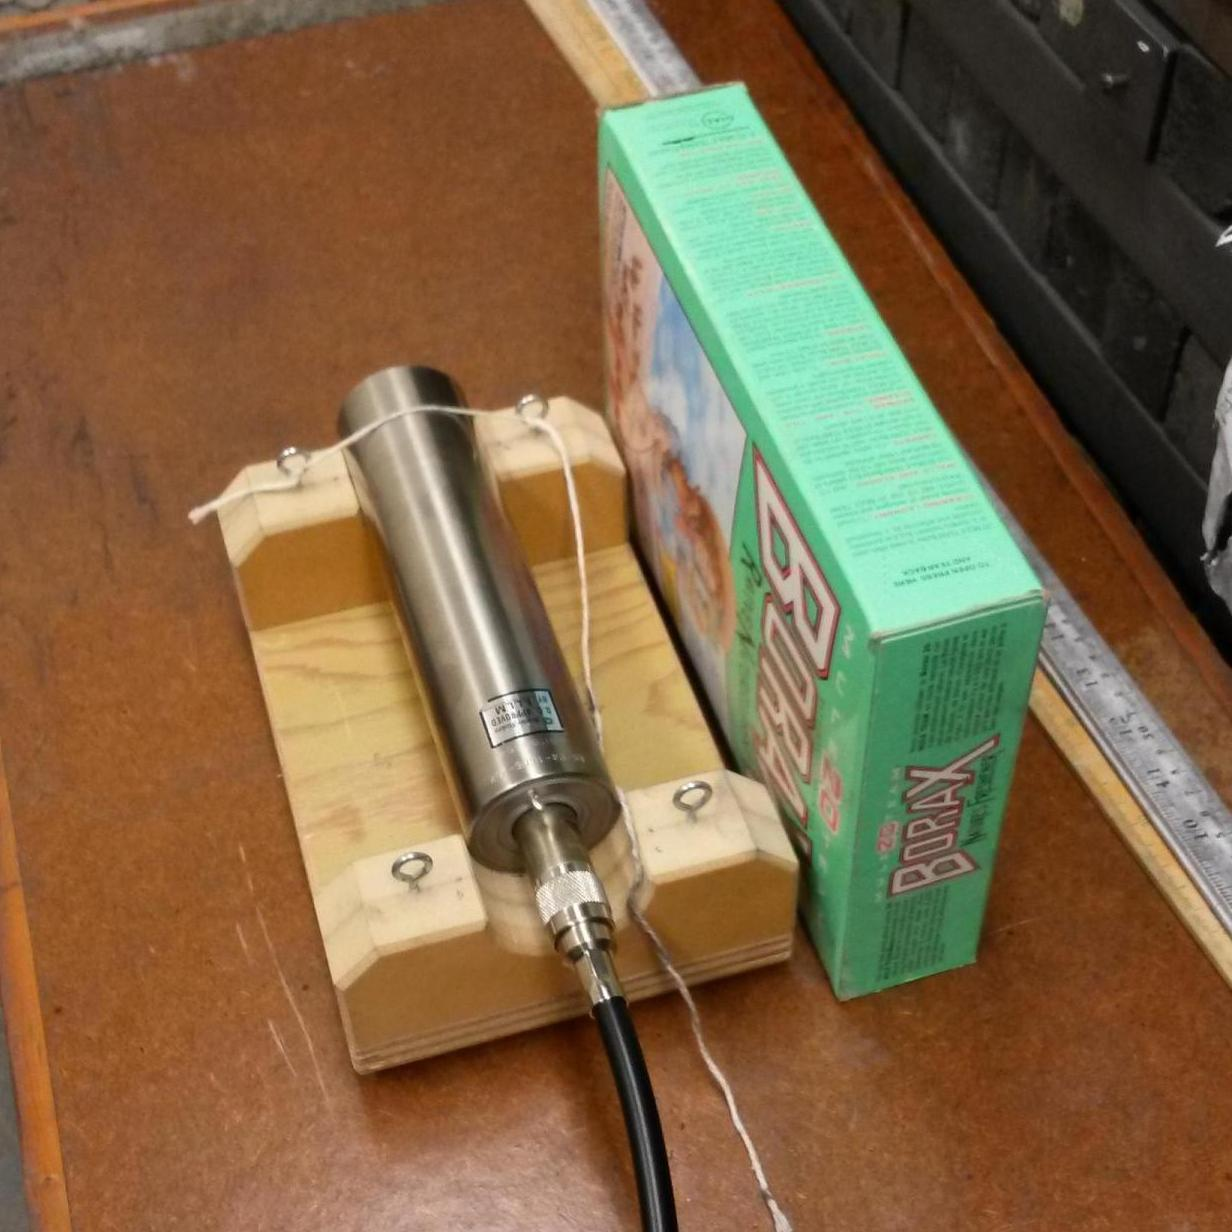
\includegraphics[scale=0.2]{images/Borax}
	}
	\subfigure[Paraffin Wax]{
		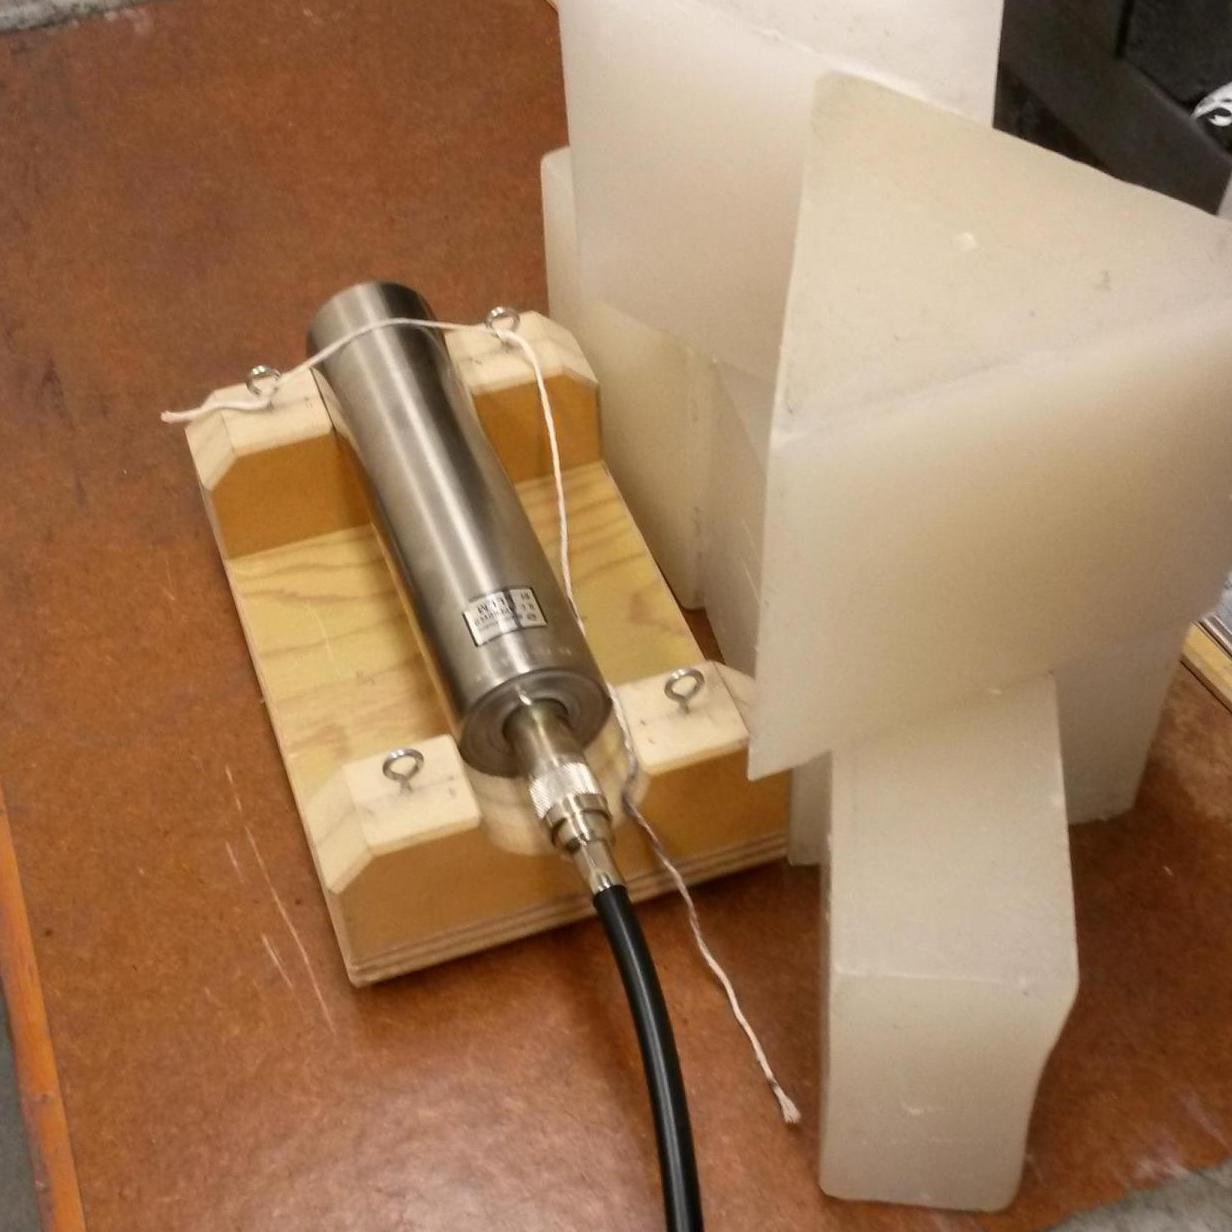
\includegraphics[scale=0.2]{images/Wax}
	}
	\subfigure[Polyethylene]{
		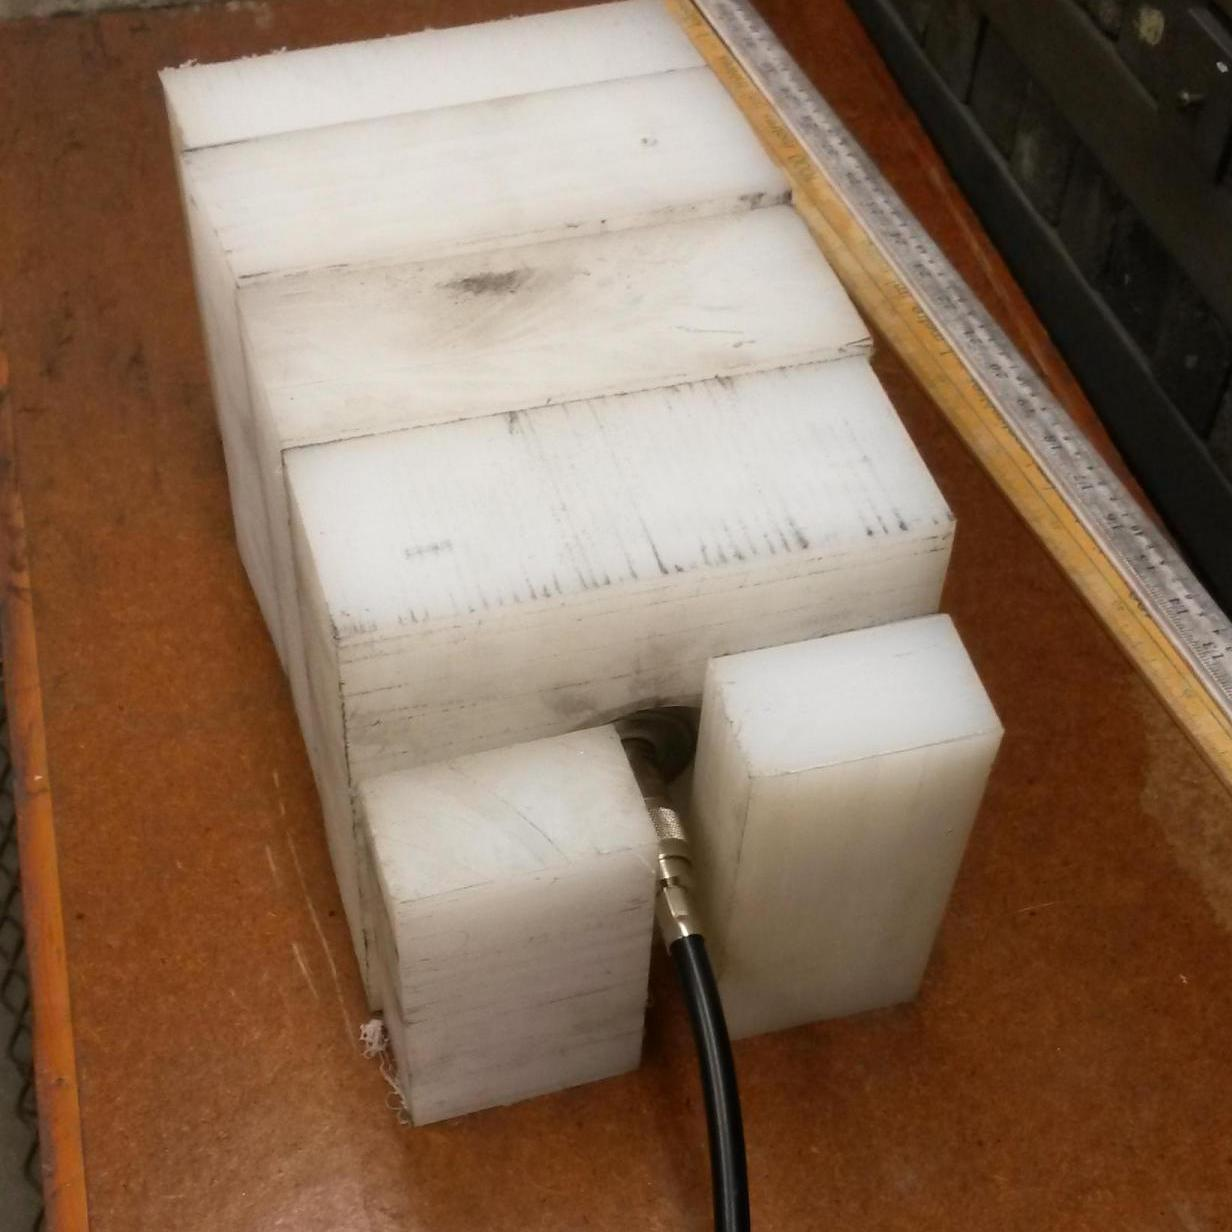
\includegraphics[scale=0.2]{images/Poly}
	}
	\subfigure[All]{
		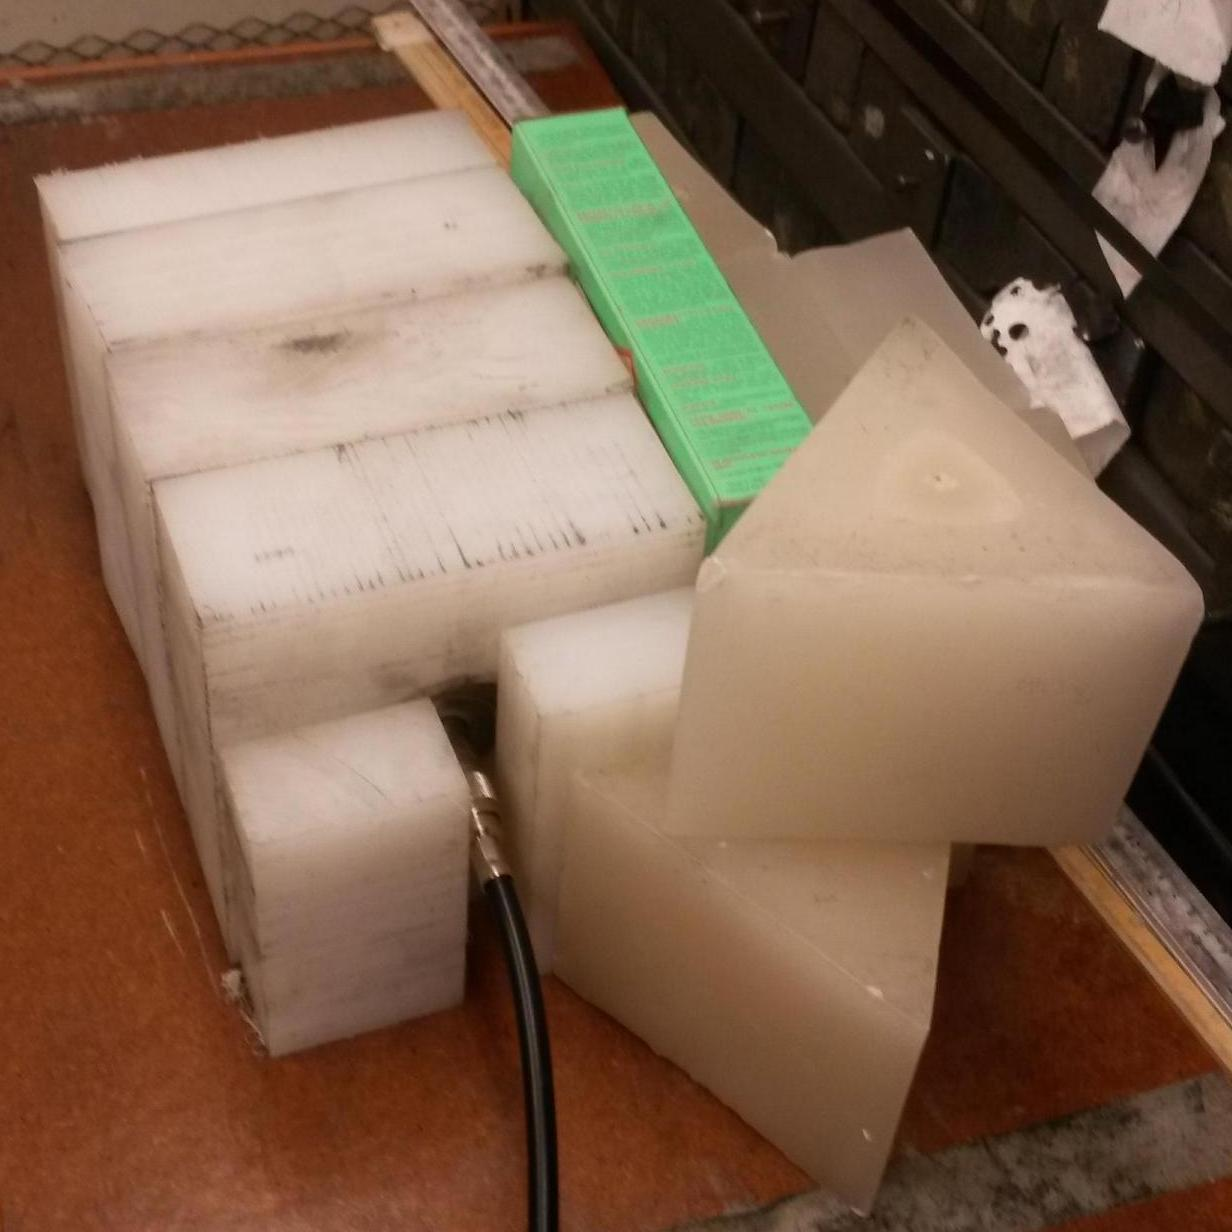
\includegraphics[scale=0.2]{images/All}
	}
	\caption{Arrangement of various shielding materials}	
	\label{fig:matTest}
\end{figure}
\clearpage


The count rate as a function of distance from the neutron source was also measured. Rate measurements were taken at 5cm increments in the distance from the source, up to 1.5m. Rate vs. distance was plotted (see Fig~\ref{fig:rateVsD}) and fitted to a $1/r^2$ function:
\begin{equation}
		{C=\frac{A_{0}}{\left ( r - r_{0} \right )^{2}}+C_{0}}
\end{equation}
Where $r_0$ and $C_0$ are offsets due to the measurements not starting at the source and the background rate being non zero. The rate follows the expected $1/r^2$ behaviour.


\begin{figure}[htb]
	\centerfloat
	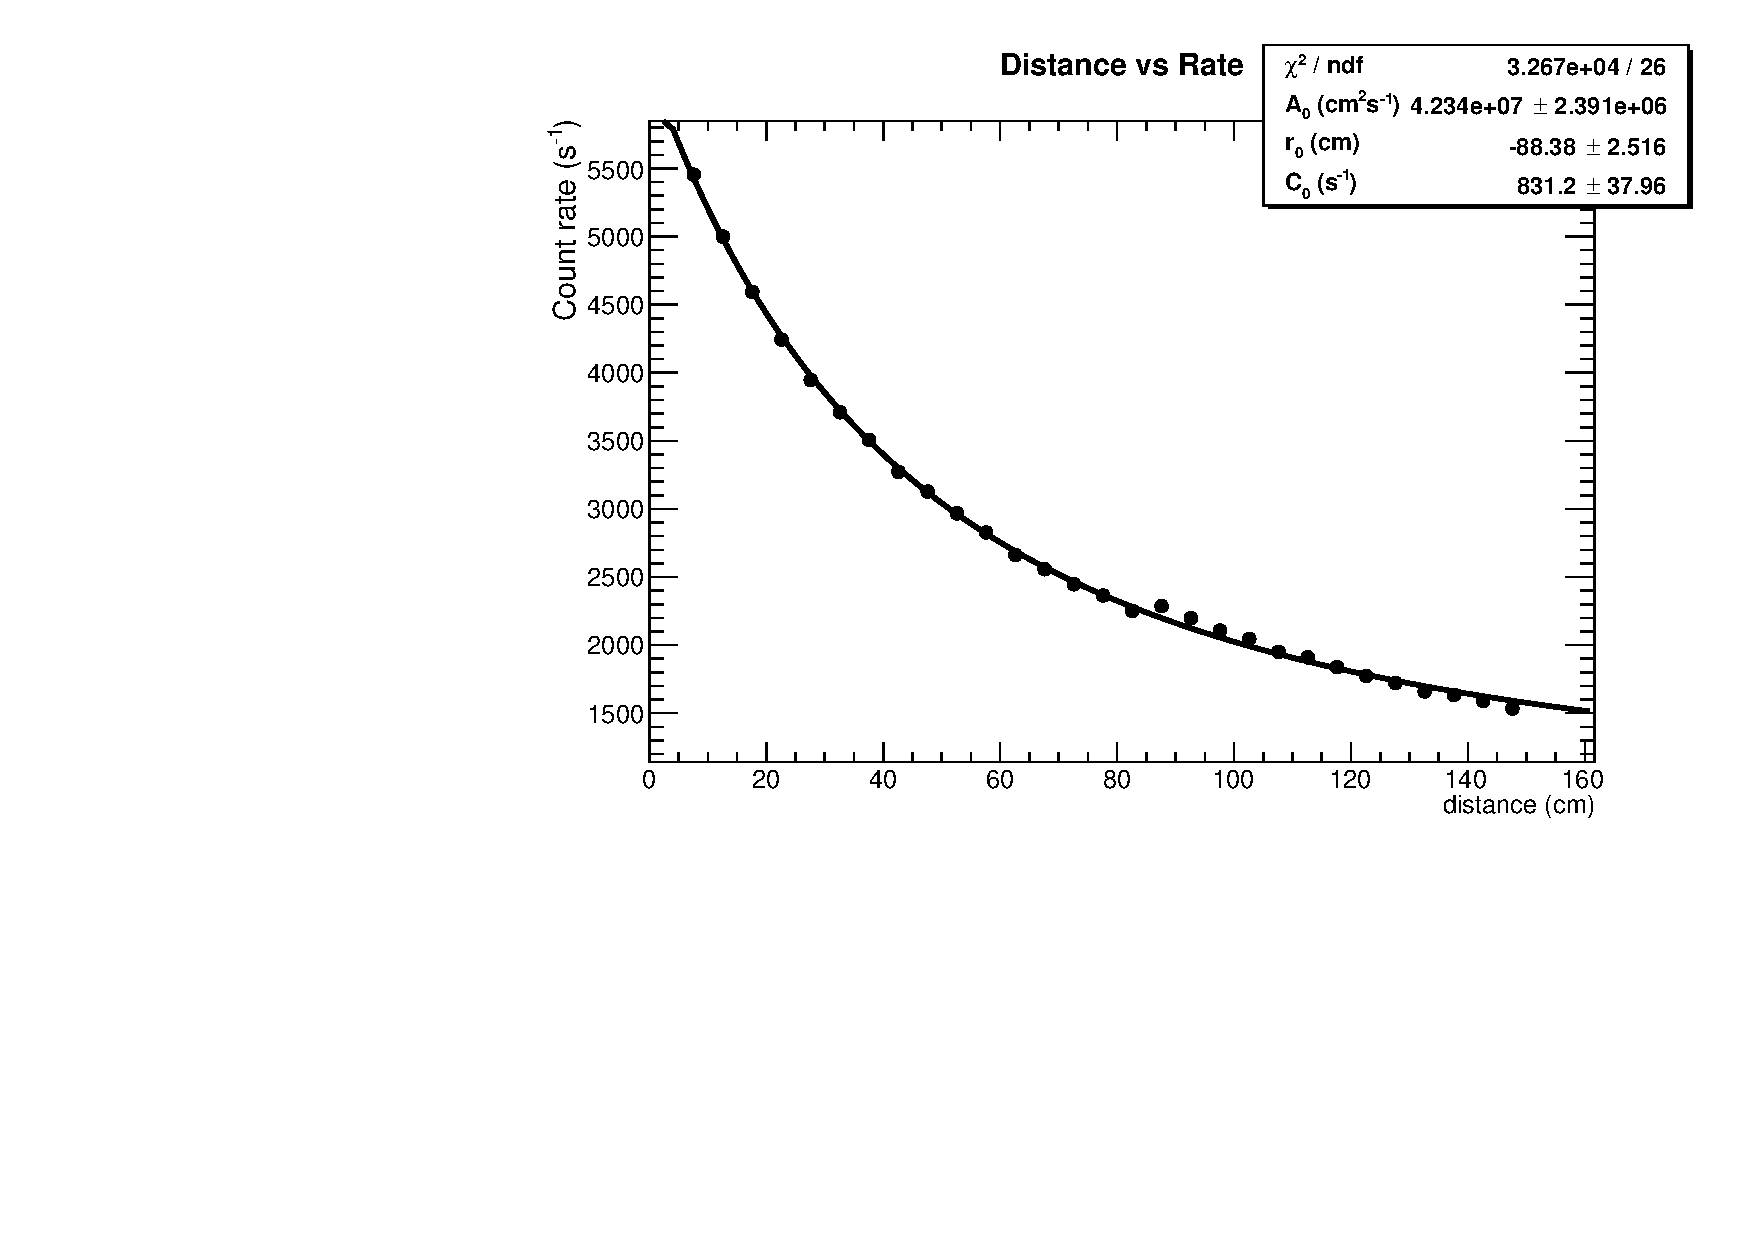
\includegraphics[width=6in]{images/rate_vs_distance_fit}
	\caption{Neutron rate vs distance from source}	
	\label{fig:rateVsD}
\end{figure}


\clearpage
\section{Preamplifiers}

	A prototype preamp was designed and built by the electronic shop in the Physics and Astronomy department at UVic.


	The final preamp design is currently being built. It will attach to the end of the He-3 tube directly, as seen in Fig~\ref{fig:preamp}. Thus, three cables will have to be routed to the tube: high voltage for the sense wire, low voltage to power the preamp, and the signal cable.





\begin{figure}[htb]
	\centering
	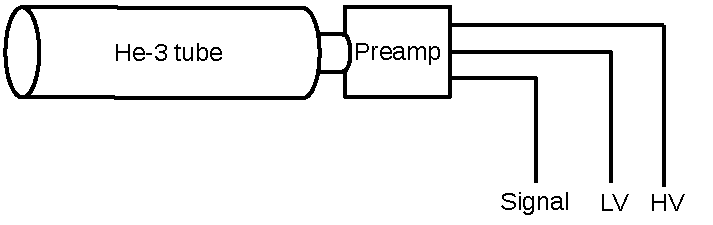
\includegraphics[width=5in]{images/preamp}
	\caption{Preamp placement}	
	\label{fig:preamp}
\end{figure}



\section{Data Acquisition}

	The data acquisition is done using a CAEN VME digitzer and a CAEN VME-USB bridge. The signal pulses from the He-3 tubes are sent to the digitizer via the preamp. The digitizer calculated the pulse height of the signal, which is then sent to the a computer, along with a time stamp, via the VME-USB bridge.

	On the software side, a DAQ program has been written that unifies the CAEN libraries with the Experimental Physics and Industrial Control System (EPICS), which is the interface that will be used to control BEAST~II. The program will be used to initialize the digitizer, start and stop the acquisition of data, and send monitoring plots to BEAST~II control room. At this point, the software is at a preliminary stage, and work is still being done on it. A schematic of the data flow from the He-3 tube to the computer can be found in Fig~\ref{fig:dataFlow}.


\begin{figure}[htb]
	\centerfloat
	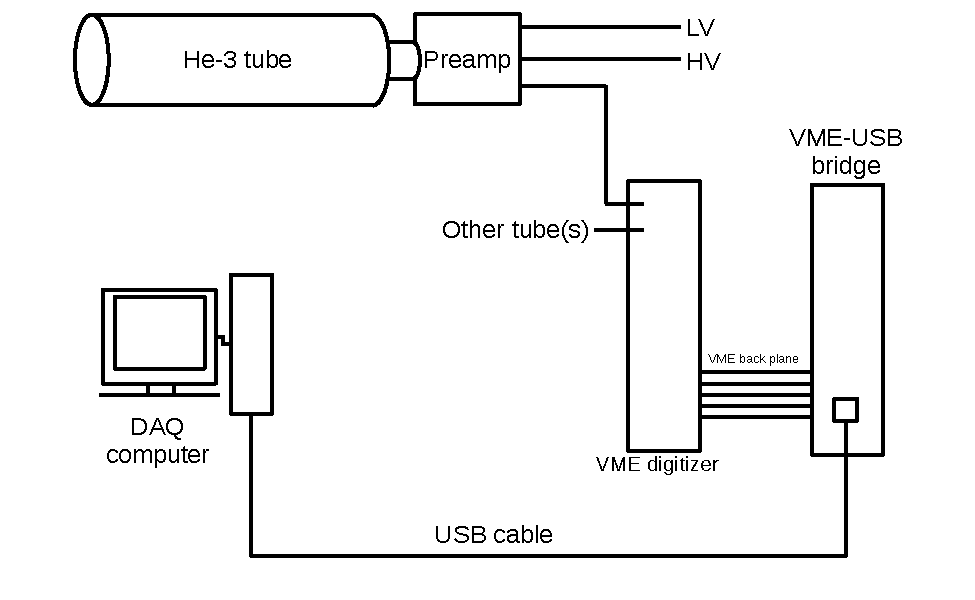
\includegraphics[width=6in]{images/DAQ-Pipeline}
	\caption{Data pipeline}	
	\label{fig:dataFlow}
\end{figure}

